\documentclass[tikz,border=3pt]{standalone}
\usepackage{amsmath}
\usepackage{tikz}
\usetikzlibrary{shapes.geometric,arrows.meta,patterns,calc,decorations.pathreplacing}

\begin{document}
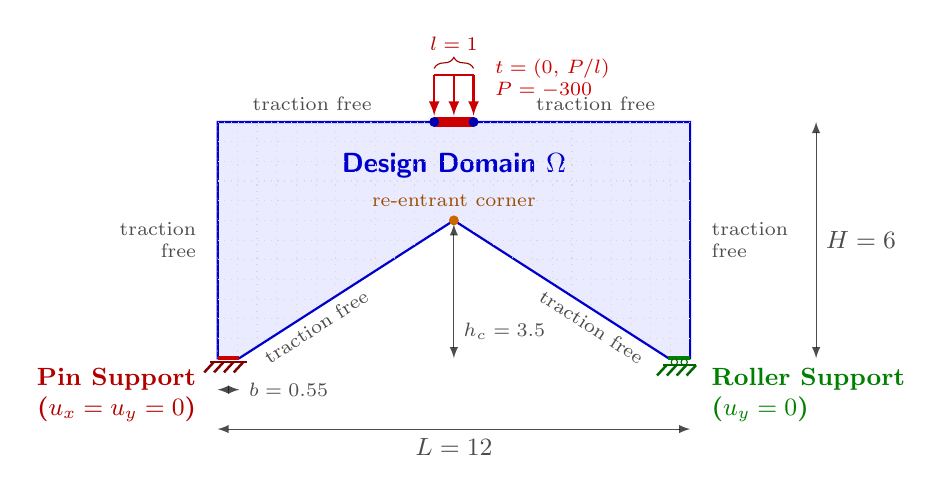
\begin{tikzpicture}[scale=1.0, >=latex]
  % PortalFramePatch2d: L x H = 12 x 6, 绘图比例 0.5 -> 6.0 x 3.0
  % b = 0.55 -> 0.275; h_c = 3.5 -> 1.75; 凹角顶点 (L/2, h_c) -> (3, 1.75)
  % 载荷区 x in [5.5, 6.5] (load_width = 1) -> 绘图 x in [2.75, 3.25]
  % Design Domain: 七边形 (0,0), (b,0), (L/2,h_c), (L-b,0), (L,0), (L,H), (0,H)
  \draw[thick, fill=blue!8, draw=blue!80!black]
    (0,0) -- (0.275,0) -- (3,1.75) -- (5.725,0) -- (6,0) -- (6,3) -- (0,3) -- cycle;
  \node[font=\bfseries\sffamily, color=blue!80!black] at (3,2.45) {Design Domain $\Omega$};

  % Grid overlay (clipped to the domain)
  \begin{scope}
    \clip (0,0) -- (0.275,0) -- (3,1.75) -- (5.725,0) -- (6,0) -- (6,3) -- (0,3) -- cycle;
    \draw[step=0.25, gray!30, dotted] (0,0) grid (6,3);
  \end{scope}

  % Re-entrant corner (L/2, h_c): geometric singularity
  \fill[orange!80!black] (3,1.75) circle (1.8pt);
  \node[above, orange!60!black, font=\scriptsize] at (3,1.8) {re-entrant corner};
  \draw[<->, opacity=0.7] (3,0) -- (3,1.7) node[pos=0.2, right, font=\scriptsize] {$h_c = 3.5$};

  % Left support segment (y = 0, x in [0, b]): pin, u_x = u_y = 0
  \draw[ultra thick, red!80!black] (0,0) -- (0.275,0);
  \draw[thick, red!50!black] (-0.1,-0.05) -- (0.375,-0.05);
  \foreach \x in {-0.05, 0.075, 0.2, 0.325} {
    \draw[line width=0.9pt, red!50!black] (\x,-0.05) -- (\x-0.12,-0.18);
  }
  \node[below left, red!70!black, font=\small\bfseries, align=right] at (-0.15,0)
    {Pin Support\\($u_x = u_y = 0$)};
  \draw[<->, opacity=0.7] (0,-0.4) -- (0.275,-0.4) node[right, font=\scriptsize] {$b = 0.55$};

  % Right support segment (y = 0, x in [L - b, L]): roller, u_y = 0
  \draw[ultra thick, green!50!black] (5.725,0) -- (6,0);
  \draw[fill=white, draw=green!40!black] (5.8,-0.05) circle (0.04);
  \draw[fill=white, draw=green!40!black] (5.925,-0.05) circle (0.04);
  \draw[thick, green!40!black] (5.65,-0.09) -- (6.075,-0.09);
  \foreach \x in {5.7, 5.825, 5.95, 6.075} {
    \draw[line width=0.9pt, green!40!black] (\x,-0.09) -- (\x-0.12,-0.22);
  }
  \node[below right, green!50!black, font=\small\bfseries, align=left] at (6.15,0)
    {Roller Support\\($u_y = 0$)};

  % Load patch on the Top Edge (y = H), x in [L/2 - l/2, L/2 + l/2]
  \draw[line width=3.5pt, red!80!black] (2.75,3) -- (3.25,3);
  \fill[blue!70!black] (2.75,3) circle (1.8pt);
  \fill[blue!70!black] (3.25,3) circle (1.8pt);
  \draw[thick, red!80!black] (2.75,3.6) -- (3.25,3.6);
  \foreach \x in {2.75, 3.0, 3.25} {
    \draw[->, thick, red!80!black] (\x,3.6) -- (\x,3.08);
  }
  \draw[decorate, decoration={brace, amplitude=4pt}, red!60!black]
    (2.75,3.68) -- (3.25,3.68) node[midway, above=3pt, font=\scriptsize, red!70!black] {$l = 1$};

  % 右侧标注: 牵引与合力
  \node[right, red!80!black, font=\scriptsize, align=left] at (3.4,3.55)
    {$t = (0,\,P/l)$\\$P = -300$};

  % Traction-free edges
  \node[above, gray!60!black, font=\scriptsize] at (1.2,3.02) {traction free};
  \node[above, gray!60!black, font=\scriptsize] at (4.8,3.02) {traction free};
  \node[left, gray!60!black, font=\scriptsize, align=right] at (-0.15,1.5) {traction\\free};
  \node[right, gray!60!black, font=\scriptsize, align=left] at (6.15,1.5) {traction\\free};
  \node[gray!60!black, font=\scriptsize, rotate=32.6] at (1.25,0.4) {traction free};
  \node[gray!60!black, font=\scriptsize, rotate=-32.6] at (4.75,0.4) {traction free};

  % Dimensions
  \draw[<->, opacity=0.7] (0,-0.9) -- (6,-0.9) node[midway, below, font=\small] {$L = 12$};
  \draw[<->, opacity=0.7] (7.6,0) -- (7.6,3) node[midway, right, font=\small] {$H = 6$};
\end{tikzpicture}
\end{document}
